\section{Algorithms}
\label{sec:algorithms}

% \red{\textit{The first part contains the detailed discussion and the
%     mathematical description of the used algorithms. The second part contains
%     the recipe algorithm, i.e. a high-level description of the recipe
%     flow-chart and how it changes for different parameter settings.}}

\subsection{General Algorithms}
\label{sec:algorithms-general}

\subsection{Optimal Extraction}
\label{sec:extract}
\begin{figure}[ht]
    \begin{center}
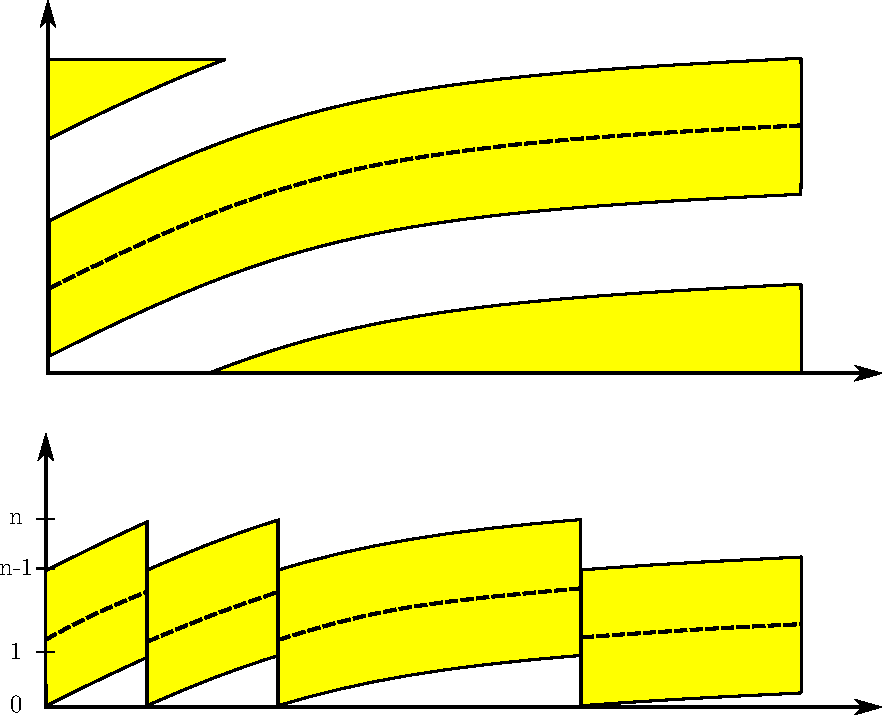
\includegraphics[width=0.45\linewidth]{rectification.pdf}
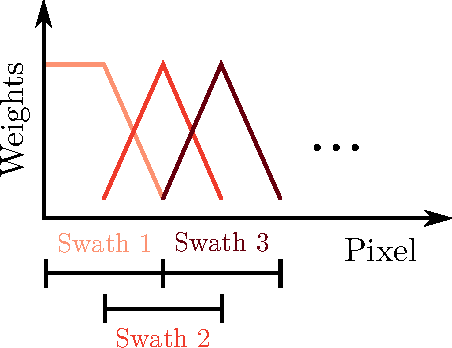
\includegraphics[width=0.45\linewidth]{swath_weights.pdf}
\end{center}
\caption{\it Left: Illustration of swath rectification. Right: The weights for combining the spectra from overlapping swaths.}
\label{fig:swaths}
\end{figure}

\begin{figure}[ht]
    \begin{center}
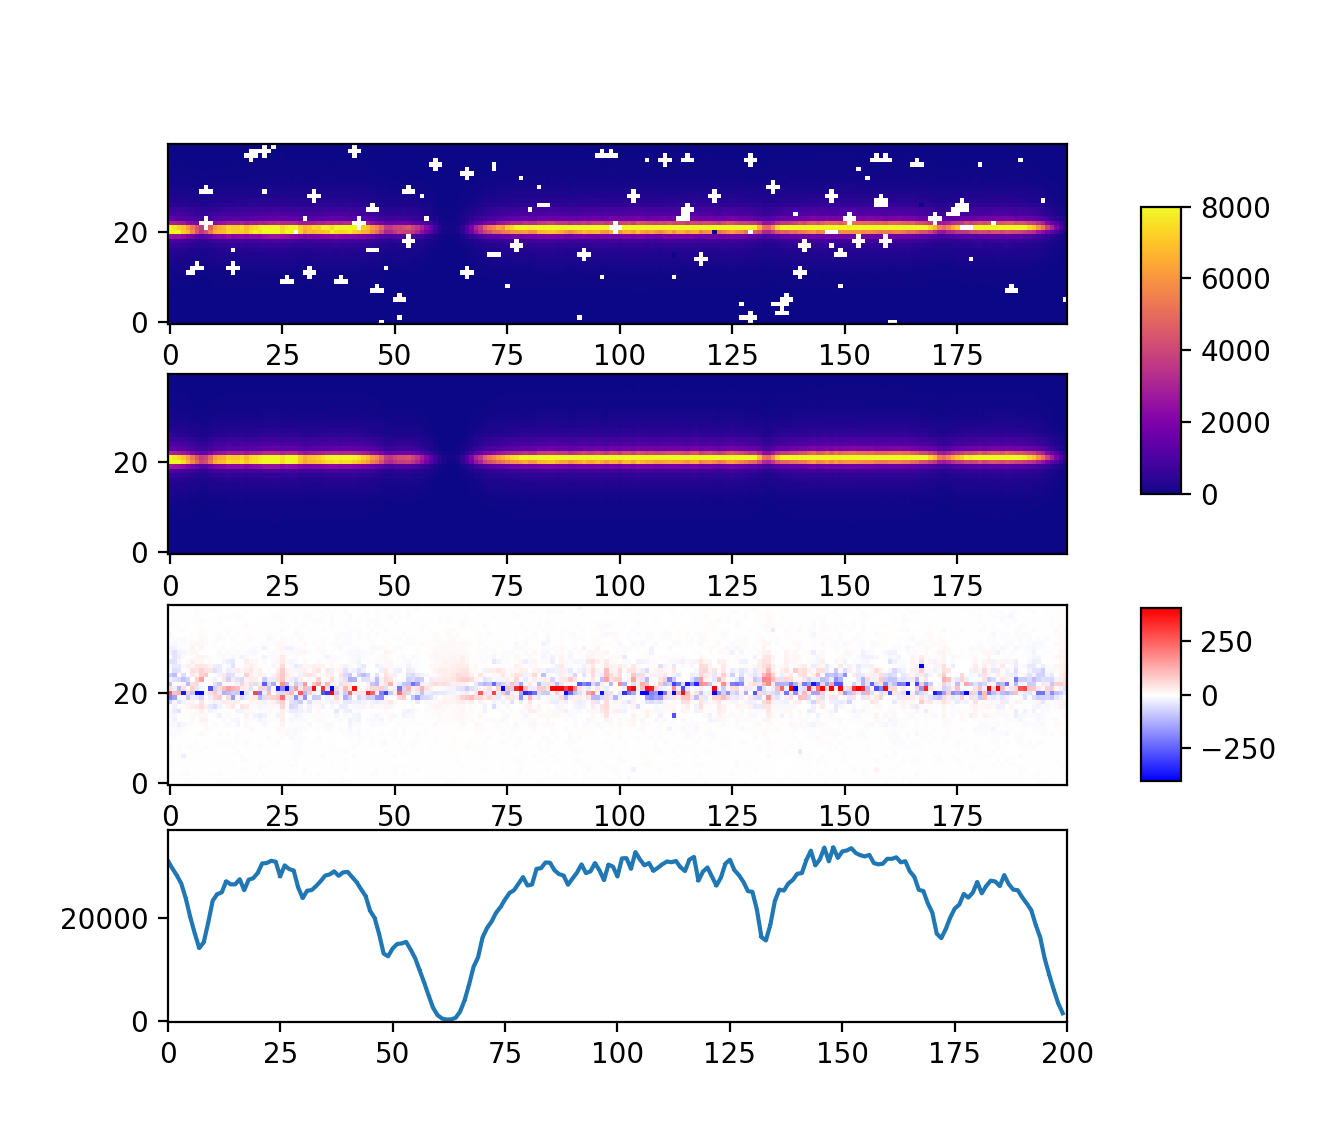
\includegraphics[width=0.85\linewidth]{extr_model.png}
\end{center}
\caption{An example of the optimal extraction. \emph{Top:} The flat-fielded,
combined, and pair-wise subtracted frame, with the BPM applied and zoomed-in to
part of a single spectral order. \emph{Panel 2:} The model of the same region,
reconstructed from the extracted spectrum and slit-function. \emph{Panel 3:} The
difference between the two above, showing the residuals. \emph{Bottom:} The extracted
spectrum itself, on the same x-axis as the panels above.}
\label{fig:extrmodel}
\end{figure}

The optimal extraction along the tilted and curved slit is a centerpiece of the
\instrument\ DRS and several recipes make use of it. Full details and
mathematical description can be found in \cite{2021A&A...646A..32P}. Here, we
simply summarize the most important practical implications from a user
perspective.

To extract a spectral order from a calibrated 2D frame into a 1D spectrum, using
a \emph{trace} from the TW table, the following steps are carried out:
\begin{itemize}
    \item Calculate the extraction height from the edge-polynomials, if not
    explicitly given via \texttt{-{}-extract\_height}.
    \item Cut out a rectangular region around the mid-line, called a
    \emph{swath} from the frame, using the height and the value of
    \texttt{-{}-extract\_swath\_width}.
    \item Rectify the swath by shifting columns by integer values such that the
    mid-line only retains values between $0\ldots 1$, like illustrated in
    \figref{fig:swaths} (left).
    \item Iteratively approximate the swath surface by two vectors: the spectrum
    along the mid-line and the slit-function along the slit projection, taking
    its changeing tilt into accont. The slit function is oversampled by a factor
    \texttt{-{}-extract\_oversample}.
    \item Step by a half swath-width to the next one, and repeat. This way
    swaths overlap fully and the order effectively gets extracted twice.
    \item Once all swaths are extracted, the spectra from each are merged into
    one, with linearly in-/decreasing weights, as in \figref{fig:swaths}
    (right).
    \item The spectrum and slit-functions are saved, and used to reconstruct a
    2D model of the frame, saved separately.
    \item The errors are estimated from the residual between data and model.
\end{itemize}

A major advantage of this extraction algorithm is that it makes not assumption
about the slit-function, except that it does not change within a swath.

In addition, the model by design cannot approximate features that are not
present in all pixels that contribute to a certain bin in the spectrum or the
slit-function. This makes spectra robust towards e.g.~cosmic rays.

\putgraph{.8\linewidth}{varyoversample.png}{varyovers}{Example spectrum,
 extracted with varying oversampling. In this case, oversampling of 12 is needed to no longer see "spiky" artifacts.}

\subsection{Errors and Signal-to-Noise}
\label{sec:errors}


The normalization of the output-spectra is like that of a sum of pixel values,
collapsed along the slit, i.e. summed-up ADU. Errors are absolute.

If \verb!NDIT >1!, then a factor of $\sqrt{NDIT}$ needs to be taken into account,
because the sub-exposured were averaged in the detector software, not affecting
the ADU level.

\subsection{Recipes Algorithms} 
\label{sec:algorithms-recipes}


%\subsection{Nodding}
%\label{sec:nodd}
%Nodding sequence \texttt{SEQ.NABCYCLES} \texttt{SEQ.NODPOS}
%first combined, then calibs applied, then subtracted, then extraction

\subsubsection{Order Tracing}
\label{sec:ordertrace}

As written above, by a \emph{trace}, we mean a polynomial, in pixel-coordinates of a single detector, that follows the mid-line of a spectral order. And two more polynomials for the upper and lower edges of the slit projection, as shown in Fig.~\ref{fig:flat_trace}.

The way this is derived is by first determining which pixels in a FLAT frame contain signal, and which don't. To that end the image is smoothed first horizontally, then vertically, and then compared to the unsmoothed frame via thresholding.

After that it is determined which spectral order the pixels belong to. For this purpose, the mean Y-coordinate for each order is present in the raw file headers.

Lastly, the pixels from the same order are fitted with a polynomial.

%smooth in x. smooth strongly in y and compare to unsmoothed, threshold. unify
%clusters. label them. threshold minimum number od pix in cluster. fit
%%polynomial to all pix. fit edges.

\subsubsection{Measuring the slit-tilt}
\label{sec:tilt}

The recipe \verb!cr2res_util_slit_curv! takes as input a TW, for the order traces, and an FPET frame. The algorithm finds the etalon peaks, which give good coverage in each spectral order.

More detail will be provided in a future iteration of this document.

\subsubsection{Wavelength calibration}

There are several ways to calibrate the wavelength scale, and each corresponds
to one of the values that the parameter \texttt{-{}-wl\_method} of
\texttt{cr2res\_util\_wave} can take.

With \texttt{-{}-wl\_method=XCORR} the provided catalog of lines gets made into
a synthetic spectrum that is cross-correlated with the extracted lamp spectrum.
Each detector-order is calibrated separately.

The recipe \texttt{cr2res\_cal\_wave} combines two methods into one recipe, one
for the UNE lamp frames, and the one for the FPET. The result from the former
gets passed on to the latter, if both lamp inputs are present. If not, then only
the appropriate method is applied.